\chapter{Entregable 3}

\section{Base de datos WINE}

Escoja una de las bases de datos de la clasificación para el trabajo de las dispuestas en Moodle.Aplique el preprocesamiento adicional (si se puede aplicar) sobre: 1) reemplazamiento de datos perdidos, 2) normalización y 3) paso de nominal a binario u ordinal a numérico.
Explique el procesamiento que haya llevado a cabo en los aspectos citados, y de no tener que hacerlo expliqué también el por qué.

Nuestro ejemplo elegido en este caso que ha sido wine.arff solo hemos tenido que normalizar los datos ya que no teníamos ningún dato perdido y además todos los atributos de nuestro fichero eran numéricos por lo que nos ha sido bastante sencillo.
\begin{figure}[H]
    \centering
    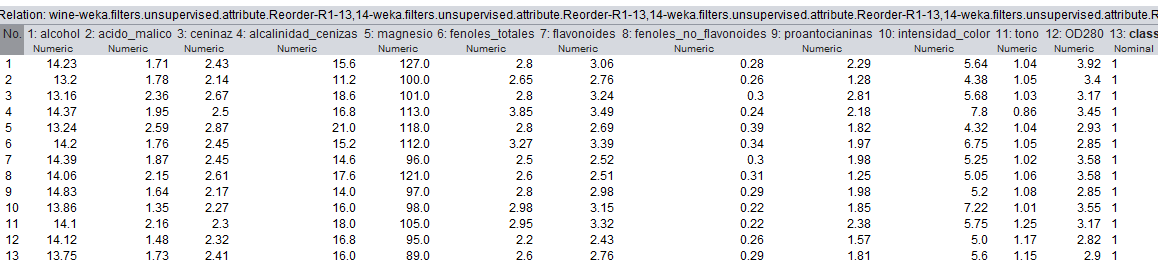
\includegraphics[width=\textwidth]{img/BNorm.PNG}
    \caption{Wine.arff antes de aplicar el filtro Normalize}
\end{figure}
Como vemos en la figura anterior los valores originales de nuestro fichero están sin organizar por lo tanton aplicaremos el filtro para conseguir que todos queden entre cero y uno.
\begin{figure}[H]
    \centering
    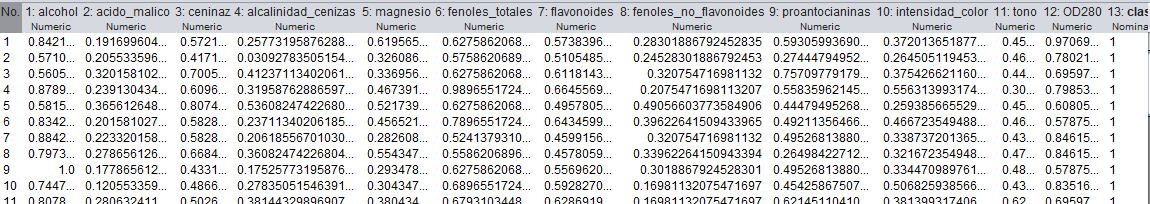
\includegraphics[width=\textwidth]{img/ANorm.PNG}
    \caption{Wine.arff una vez normalizado}
\end{figure}


\subsection{Algoritmo clasificación KNN}
Con la base de datos escogida anteriormente, use el algoritmo de clasificación KNN con un 10-fold crossvalidation. Use un valor de vecinos k=3 dejando por defecto el resto de parámetros.

Para realizar este ejercicio una vez ya tenemos preprocesada nuestra base de datos, nos vamos al apartado classify dentro de Weka, una vez aquí escogemos nuestro clasificador deseado, en este caso vamos a utilizar el clasificador KNN, conocido como algoritmo del vecino más cercano, para ello debemos de entrar dentro de la carpeta lazy en el cual se encuentra y seleccionar el clasificador ibk que es el nombre asignado en Weka para nuestro algoritmo. Una vez seleccionado debemos de modificar algunos valores por defecto ya que por defecto el numero de vecinos con el que comparar en uno es decir k=1, para nuestro problema en concreto tal y como nos indica en el enunciado debemos de cambiarlo y usar k=3, y además utilizar crossvalidation con 10 folds tal y como se muestra en la figura de abajo.

\begin{figure}[H]
    \centering
    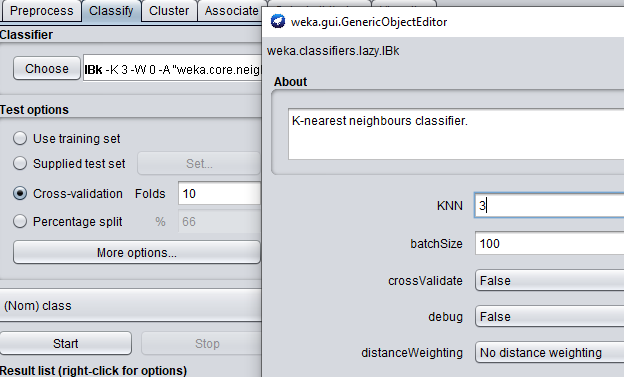
\includegraphics[width=\textwidth]{img/IB3.PNG}
    \caption{Valores modificados para IBK, k=3}
\end{figure}

Una vez aplicado el clasificador sobre nuestra base de datos vemos como han sido los resultados:
\begin{figure}[H]
    \centering
    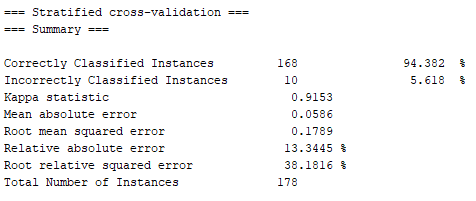
\includegraphics[width=\textwidth]{img/EGlobales.PNG}
    \caption{Estadísticas globales de nuestro clasificador}
\end{figure}

Nuestro clasificador ha realizado una muy buena clasificación obteniendo un total de 168 instancias bien clasificadas de las 178 totales con solo 10 erróneas.
Ha conseguido un 94.382\% de instancias bien clasificadas, frente a un 5.618\% de instancias mal clasificadas.

\begin{figure}[H]
    \centering
    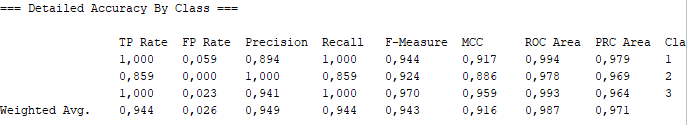
\includegraphics[width=\textwidth]{img/Ebyclass.PNG}
    \caption{Estadísticas de clasificación de cada clase}
\end{figure}

En la figura de arriba vemos una tabla en la cual nos da datos referentes a la clasificación más detallada de cada clase, cabe destacar los valores de TP Rate de la clase uno y dos(valores de uno para ambas clases) en  las cuales todas las instancias han sido clasificadas de manera correcta, además debemos de tener en cuenta la media de ROC Área que es muy cercana a uno la cual nos indica que nuestro clasificador está muy bien entrenado.

En la siguiente figura, la matriz de confusión, nos indica como se han clasificado las instancias en cada clase, vemos como lógicamente coincide con lo comentado anteriormente y en la clase a(1) y c(3) todas las instancias han sido clasificadas de manera correcta, mientras que en la clase b(2) de las 71 instancias pertenecientes a esta clase ha sido bien clasificadas 61, siendo de estas 7 clasificadas de manera errónea en la clase a(1) y 3 en la clase c(3).

\begin{figure}[H]
    \centering
    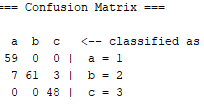
\includegraphics[width=0.9\textwidth]{img/MConf.PNG}
    \caption{Estadísticas de clasificación de cada clase}
\end{figure}


\subsection{Algoritmo Simple Logistic}
Con la base de datos escogida anteriormente, ejecute el algoritmo SimpleLogistic con 10-fold crossvalidation. 


\begin{figure}[H]
    \centering
    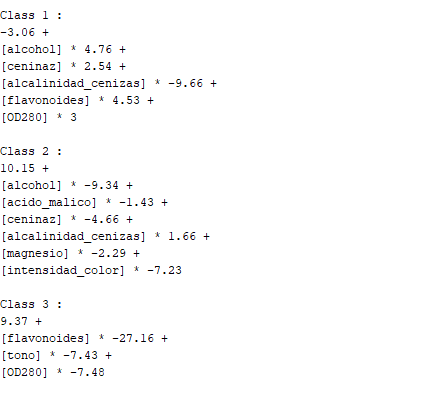
\includegraphics[width=\textwidth]{img/SL.PNG}
    \caption{Modelo de Regresión Logística obtenido al aplicar SampleLogistic}
    \label{fig:Modeloregresion}
\end{figure}
    
Una vez cargada nuestra base de datos Wine en Weka y preprocesada correctamente entramos en el apartado Classify para aplicar el algoritmo de regresión SampleLogistic, para ello entramos dentro de la carpeta functions que se encuentra a su vez dentro de la carpeta clasifiers y seleccionamos nuestro algoritmo.
En el resultado obtenido tal y como se indica en la figura de abajo nos aparece las distintas rectas de regresión obtenidas por el modelo, a partir de estas rectas mediante la función softmax obtenemos la probabilidad de pertenencia de una instancia a una de las clases. Además observamos (Fig\ref{fig:Modeloregresion}) como hay algunos atributos que no aparecen en estas funciones por lo tanto no son de utilidad a la hora de clasificar una instancia, estos atributos son, fenolestotales, fenolesnoflavonoides, proantocianinas.


En las siguientes ecuaciones que indican las rectas de regresión de las distintas clases vemos los valores de beta los cuales indican la importancia de las variables.Todas siguen la siguiente ecuación:

A continuación se expone la recta de regresión de la clase uno donde vemos que las variables que mas influyen son alcalinidad\_cenizas y alcohol. $f_1(x,\theta)=-3.06+Alcohol\ast4.76+ceninaz\ast2.54+alcalinidad\_cenizas\ast-9.66+flavonoides\ast4.53+OD280\ast3$

La siguiente ecuación \ref{ecuacion} nos muestra la recta de regresión de la clase dos donde debemos destacar que las variables mas influyentes son intensidad\_color y alcohol.

\begin{equation}
	f_1(X,\hat{\theta}) = \beta_0 + \sum_{i=1}^{n} \hat{\beta_i}x_i
	\label{ecuacion}
\end{equation}


$ f_2(x,\theta)=10.15+Alcohol\ast9.34+ceninaz\ast-4.66+alcalinidadcenizas\ast1.66+acidomalico\ast-1.43+magnesio\ast-2.29+intensidadcolor\ast-7.23 $


Por último tenemos la ecuación de regresión de la clase tres en la que destaca la importancia de la variable flavonoides.

$ f_3(x,\theta)=9.37+Flavonoides\ast-27.16+tono\ast-7.43+OD280\ast-7.48 $

Con respecto a las métricas se tiene un CCR 95.5056 de un  frente 94.38 al de un que daba el algoritmo KNN. El estadístico kappa 0.932 es igual a que como en el caso anterior quiere decir que el modelo obtenido es muy superior que uno basado en el azar. Por otro lado los valores de TP rate por clase son 0.983, 0.901 y 1 que son bastante similares a los obtenidos anteriormente. 

\begin{figure}[H]
    \centering
    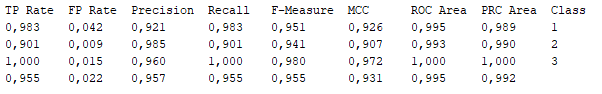
\includegraphics[width=\textwidth]{img/SLbyClass.PNG}
    \caption{Estadísticas de clasificación de cada clase}
    
\end{figure}